
% BEGIN COMPLETE NATIVE TRACE ACTION PROOFS

\clearpage\begingroup
\part*{The outgoing arithmetic relation: complete spectral action}
\newcommand{\sapC}{\mathbb C}\newcommand{\sapR}{\mathbb R}
\newcommand{\saptr}{\operatorname{tr}}\newcommand{\sapRes}{\operatorname{Res}}
\newcommand{\sapid}{\operatorname{Id}}\newcommand{\sapdd}{\dagger_G}
\newtheorem{saptheorem}{Theorem}[section]
\newtheorem{saplemma}[saptheorem]{Lemma}


\section{Objects, source use and scope}

Connes and van Suijlekom \cite{sap:CV}, Section \texttt{sect:sa},
apply divided differences to a trace action with a rank-one,
not necessarily selfadjoint perturbation. Here that calculation
is carried out for the original attained arithmetic quotient
and its outgoing relation. Every trace below is finite.
The test function $F$ is an arbitrary polynomial, so every
expansion in its perturbation parameter terminates. No
infinite trace, spectral limit or Riemann-hypothesis endpoint
is inferred.

Retain the actual packet, with complete zero orders, and
the original arithmetic source:
\begin{equation}\tag{SA1}\label{sap:SA1}
\begin{gathered}
h(s)=\prod_{\rho\in Z}(s-\rho)^{m_\rho},\qquad
g(s)=2\xi(s)=s(s-1)\pi^{-s/2}\Gamma(s/2)\zeta(s),\\
\mathcal MF_h=g/h,\qquad
w_h(v)=\frac{|(g/h)(1/2+iv)|^2}{2\pi},\qquad
m(u)=w_h^{*k}(u),\qquad c=k/2,\quad S=c+iu.
\end{gathered}
\end{equation}
The original nonempty packet is stable under conjugation
and $s\mapsto1-s$. The measure is the one in \cite{sap:Native},
NS1--NS3, not a selected comparison measure. In particular
it is even, positive almost everywhere, has every polynomial
moment, and has mass
$\mathfrak m=(\int_\sapR w_h)^k$, which is retained.
Let $Q_n$ be its real monic orthogonal polynomials and put
\begin{equation}\tag{SA2}\label{sap:SA2}
\omega_n=\int_\sapR Q_n(u)^2m(u)\,du,\quad
p_n(S)=i^nQ_n((S-c)/i),\quad
\omega_0=\mathfrak m,\quad
a_n=\sqrt{\omega_{n+1}/\omega_n}.
\end{equation}
All $\omega_n$ are strictly positive: a nonzero polynomial
cannot vanish almost everywhere for this measure.
Gram--Schmidt and evenness give
$Q_n(-u)=(-1)^nQ_n(u)$ and
$uQ_n=Q_{n+1}+(\omega_n/\omega_{n-1})Q_{n-1}$.
For the last assertion, pair with $Q_j$ for $j<n-1$,
transfer $u$ to $Q_j$, and use orthogonality; parity removes
the $Q_n$ coefficient and the $Q_{n-1}$ pairing gives
the displayed coefficient.

Let $C=\sapC[S]/(\chi)$ be the original cyclic algebra,
$q=\deg\chi$, and $M_S$ multiplication by $S$.
The full annihilator, including sum collisions, is
\begin{equation}\tag{SA3}\label{sap:SA3}
\chi(S)=\prod_\kappa(S-\kappa)^{e_\kappa},
\qquad
e_\kappa=\max_{\sum_j\rho_j=\kappa}
\left(1+\sum_{j=1}^k(m_{\rho_j}-1)\right).
\end{equation}
Indeed the local tensor ring has coordinates $z_j$ with
$z_j^{m_{\rho_j}}=0$, and the highest nonzero power of
$\sum z_j$ has coefficient
$(\sum(m_{\rho_j}-1))!/\prod(m_{\rho_j}-1)!$ on
$\prod z_j^{m_{\rho_j}-1}$. This proves the exponent and,
by taking the maximum at equal sums, the full cyclic kernel.
Set
\begin{equation}\tag{SA4}\label{sap:SA4}
M=(M_S-cI)/i,\quad
\chi_u(z)=i^{-q}\chi(c+iz)=\det(zI-M),\quad b_n=[p_n]_\chi.
\end{equation}
The determinant assertion follows from the companion
matrix of multiplication in the increasing-power basis.
Fix $L\geq q-1$ and use this original remainder basis
throughout unless a coordinate map is explicitly stated.
The attained metric and lifting maps are
\begin{equation}\tag{SA5}\label{sap:SA5}
E=\left[\frac{i^{-n}b_n}{\sqrt{\omega_n}}\right]_{n=0}^L,\quad
G=(EE^*)^{-1},\quad R=E^*G,\quad ER=I,\quad R^*R=G.
\end{equation}
The first $q$ monic columns make $E$ onto. Every lift of
$v$ is $Rv+z$, $Ez=0$, and
$\|Rv+z\|^2=v^*Gv+\|z\|^2$, since
$(Rv)^*z=v^*GEz=0$. Thus $G$ is precisely the least-norm
quotient metric, including the original mass.

Let $J_L$ be the $(L+1)$-square Jacobi matrix in the
orthonormal coordinates $Q_n/\sqrt{\omega_n}$.
Define the following \emph{different} operators on the
\emph{same} algebra and prove their exact relation:
\begin{equation}\tag{SA6}\label{sap:SA6}
A=EJ_LR=M+Q,\qquad
Q=r\ell,\qquad
r=\frac{i}{\omega_L}b_{L+1},\quad \ell=b_L^*G.
\end{equation}
To check the sign, multiplication by $u$ has its extra
outgoing column $a_Le_{L+1}e_L^*$. Removing that column
after reduction and lifting subtracts
\[
a_L\frac{i^{-(L+1)}b_{L+1}}{\sqrt{\omega_{L+1}}}
\frac{i^Lb_L^*G}{\sqrt{\omega_L}}
=-\frac{i}{\omega_L}b_{L+1}b_L^*G.
\]
This proves \eqref{sap:SA6}. Moreover $GA=R^*J_LR$ is
Hermitian, so $A^{\sapdd}=A$, where $X^{\sapdd}=G^{-1}X^*G$.
Conjugation by $G^{1/2}$ proves that $A$ has real spectrum
and a complete $G$-orthonormal eigenbasis.

The parity map $\Gamma[P(S)]=[P(k-S)]$ is well-defined
on $C$ by packet symmetry. Its entries are
$\Gamma_{rj}=\binom jr k^{j-r}(-1)^r$, $0\leq r\leq j<q$.
It satisfies
\begin{equation}\tag{SA7}\label{sap:SA7}
\Gamma^2=I,\quad \Gamma^*G\Gamma=G,\quad
\Gamma A\Gamma=-A,\quad \Gamma Q\Gamma=-Q,\quad
\ell r=0,\quad Q^2=0.
\end{equation}
For proof, $\Gamma b_n=(-1)^nb_n$, and hence
$\Gamma E=E\operatorname{diag}((-1)^n)$.
Use \eqref{sap:SA5} and the odd Jacobi matrix to prove the
first four identities. Opposite parity gives
$b_L^*Gb_{L+1}=-b_L^*Gb_{L+1}=0$, proving the last two.
This is a calculation of the pairing, not removal of a
cross term.

\section{Polynomial first principles and every repeated node}

For a polynomial $f$ define divided differences at any
nodes, including repetitions, by linearity and
\begin{equation}\tag{SA8}\label{sap:SA8}
(x^m)[x_1,\ldots,x_n]=
\begin{cases}
\displaystyle\sum_{\substack{a_1,\ldots,a_n\geq0\\
 \sum a_j=m-n+1}}\prod_{j=1}^n x_j^{a_j},&m\geq n-1,\\
0,&m<n-1.
\end{cases}
\end{equation}
This agrees with the recursive divided difference:
subtract the complete homogeneous sums with first or last
variable omitted and factor the difference of the two
powers by the difference of those variables. Induction
on $n$ starts with $f[x_1]=f(x_1)$.
The resulting polynomial identity also proves the unique
continuous extension to coincident nodes. In particular
$f[x,\ldots,x]=f^{(n-1)}(x)/(n-1)!$.
The elementary Laurent identity behind this definition is
\begin{equation}\tag{SA9}\label{sap:SA9}
\sapRes_\infty^+\frac{f(z)}
 {\prod_{j=1}^n(z-x_j)}
=f[x_1,\ldots,x_n],
\end{equation}
where $\sapRes_\infty^+$ denotes the coefficient of $z^{-1}$
in the expansion at infinity, not its negative.
Expand each $(z-x_j)^{-1}$ as a geometric series to obtain
\eqref{sap:SA8}, proving \eqref{sap:SA9} also at repeated nodes.

\begin{saptheorem}[Exact cyclic trace coefficient]\label{sap:thm:cyclic}
Let $A$ be the operator in \eqref{sap:SA6}, let $V$ be any
operator on the same finite space, and let
$A=\sum_{\lambda\in\Lambda}\lambda P_\lambda$ be its
decomposition into distinct real eigenvalues, with the
complete spectral projections. For every polynomial $F$
and $n\geq1$,
\begin{equation}\tag{SA10}\label{sap:SA10}
\left.\frac{d^n}{dt^n}\saptr F(A+tV)\right|_{t=0}
=(n-1)!\sum_{\lambda_1,\ldots,\lambda_n\in\Lambda}
F'[\lambda_1,\ldots,\lambda_n]\,
\saptr(P_{\lambda_1}V\cdots P_{\lambda_n}V).
\end{equation}
Every multiplicity of $A$ is retained inside its projector.
\end{saptheorem}
\begin{proof}
First take $F(x)=x^m$. The product rule and cyclicity give
$d\,\saptr(A+tV)^m/dt=m\,\saptr((A+tV)^{m-1}V)$:
the $m$ differentiated words have equal trace by cyclic
permutation. The coefficient of $t^{n-1}$ in the right
side is
\[
m\sum_{a_1+\cdots+a_n=m-n}
\saptr(A^{a_1}V A^{a_2}V\cdots A^{a_n}V).
\]
Insert the complete projector decomposition of each power.
The sum over exponents is exactly the divided difference
of $F'=mx^{m-1}$ on $n$ nodes, by \eqref{sap:SA8}.
Since differentiating a coefficient of $t^n$ multiplies
it by $n$, the coefficient in the trace is $1/n$ times
this sum. Multiplication by $n!$ proves \eqref{sap:SA10}.
Linearity proves the result for all $F$. Every operation
was a finite polynomial operation, so repetitions and
zero eigenvalues require no limiting argument.
\end{proof}

The statement of \cite{sap:CV}, Lemma \texttt{lem:sa}, displays
$n!$ rather than $(n-1)!$ for the sum in \eqref{sap:SA10}.
The proof there instead ends with the correct repeated-node
expression
\[
n!\sum\saptr(P_1V\cdots P_nV)F[\lambda_1,\ldots,\lambda_n,\lambda_1].
\]
Here is the exact passage between them. By \eqref{sap:SA9},
differentiation of $\prod(z-\lambda_j)^{-1}$ and extraction
of the coefficient of a derivative of a Laurent series give
\begin{equation}\tag{SA11}\label{sap:SA11}
F'[\lambda_1,\ldots,\lambda_n]
=\sum_{j=1}^n
F[\lambda_1,\ldots,\lambda_n,\lambda_j].
\end{equation}
In the full cyclic sum the $n$ summands on the right
have equal summed values, by cyclic relabelling.
Thus the repeated-node expression is $n!/n=(n-1)!$
times the $F'$ expression. The source's subsequent
second-derivative formula and Proposition
\texttt{prop:der-sa} use the latter, correct second
derivative. For an immediate coefficient test, take
dimension one, $A=0$, $V=1$, $F(x)=x^2$: the second
derivative is $2$, whereas the displayed $n!F'[0,0]$
would give $4$. No other assertion of that source is
needed for this finite correction.

\section{The complete native path, determinant and resolvent}

Return to the actual $Q=r\ell$ in \eqref{sap:SA6} and define
\begin{equation}\tag{SA12}\label{sap:SA12}
T(t)=A-tQ,\quad T(0)=A,\quad T(1)=M,\qquad
d(z)=\det(zI-A),\quad
\kappa(z)=\ell(zI-A)^{-1}r.
\end{equation}
The parameter $t$ is an algebraic perturbation parameter;
all identities of polynomials below hold for every complex
$t$. The $G$-adjoint statements later use real $t$.
Put $n(z)=\ell\,\operatorname{adj}(zI-A)r$.
The full, uncancelled characteristic polynomial is
\begin{equation}\tag{SA13}\label{sap:SA13}
\begin{split}
p_t(z)&=\det(zI-T(t))=d(z)+t n(z)
       =d(z)(1+t\kappa(z))\\
      &=(1-t)d(z)+t\chi_u(z),\qquad
n(z)=\chi_u(z)-d(z).
\end{split}
\end{equation}
For proof, away from the spectrum of $A$, factor
$zI-T=(zI-A)(I+t(zI-A)^{-1}r\ell)$ and use
$\det(I+v\ell)=1+\ell v$. A basis beginning with $v$
proves this last identity when $v\ne0$; the zero case is
immediate. Multiplication by $d$ gives a polynomial
identity everywhere. Setting $t=1$ gives the last line.
No common factor or invisible eigenvalue was removed.

For all points where the displayed inverses exist, direct
multiplication gives
\begin{equation}\tag{SA14}\label{sap:SA14}
(zI-T(t))^{-1}
=(zI-A)^{-1}
-\frac{t(zI-A)^{-1}r\ell(zI-A)^{-1}}
       {1+t\kappa(z)}.
\end{equation}
It is also an identity of rational matrices.
Taking its trace and using
$\kappa'(z)=-\ell(zI-A)^{-2}r$ yields
\begin{equation}\tag{SA15}\label{sap:SA15}
\saptr(zI-T(t))^{-1}-\saptr(zI-A)^{-1}
=\frac{t\kappa'(z)}{1+t\kappa(z)}
=\partial_z\log(1+t\kappa(z)).
\end{equation}
The logarithm is unambiguously its expansion tending to
zero at infinity. Its derivative is rational, so the
identity has no branch dependence.

Write $w_\lambda=\ell P_\lambda r$. The full scalar
resolvent and its moments are
\begin{equation}\tag{SA16}\label{sap:SA16}
\kappa(z)=\sum_{\lambda\in\Lambda}
\frac{w_\lambda}{z-\lambda}
=\sum_{j\geq0}\frac{\ell A^jr}{z^{j+1}},
\qquad \sum_\lambda w_\lambda=\ell r=0.
\end{equation}
Spectral projectors are in the original metric. Explicitly,
if $U_\lambda$ contains a basis of the eigenspace, then
$P_\lambda=U_\lambda(U_\lambda^*GU_\lambda)^{-1}
U_\lambda^*G$. Distinct eigenspaces are $G$-orthogonal
by selfadjointness, proving this expression and the
completeness used above.

\begin{saptheorem}[Trace, determinant and residue are the same calculation]
For every polynomial $F$ of degree $m$,
\begin{equation}\tag{SA17}\label{sap:SA17}
\begin{split}
\saptr F(T(t))-\saptr F(A)
&=-\sapRes_\infty^+ F'(z)\log(1+t\kappa(z))\\
&=\sum_{n=1}^{m}\frac{(-t)^n}{n}
\sapRes_\infty^+ F'(z)\kappa(z)^n\\
&=\sum_{n=1}^{m}\frac{(-t)^n}{n}
\sum_{\lambda_1,\ldots,\lambda_n}
F'[\lambda_1,\ldots,\lambda_n]\prod_{j=1}^n w_{\lambda_j}.
\end{split}
\end{equation}
\end{saptheorem}
\begin{proof}
Expand the resolvent at infinity as
$\sum_{j\geq0}T^jz^{-j-1}$. The coefficient of $z^{-1}$
in $F(z)(zI-T)^{-1}$ is $F(T)$.
Use \eqref{sap:SA15} and take its trace to obtain the first
line after integration by parts in Laurent series:
the coefficient of $z^{-1}$ of any derivative is zero.
Since $\kappa=O(z^{-1})$, terms $n>m$ cannot contribute.
The logarithm series therefore gives the second line
as a finite polynomial identity in $t$, even though its
auxiliary series is local at infinity. Insert
\eqref{sap:SA16} and apply \eqref{sap:SA9} for the third line.
Alternatively each trace cycle in \eqref{sap:SA10} for
$V=-r\ell$ is $(-1)^n\prod_j\ell P_{\lambda_j}r$.
Thus the two independent finite derivations agree.
\end{proof}

The original parity strengthens these formulas:
\begin{equation}\tag{SA18}\label{sap:SA18}
w_{-\lambda}=-w_\lambda,\quad w_0=0,\quad
\kappa(-z)=\kappa(z),\quad
\kappa(z)=\sum_{j\geq0}\frac{\ell A^{2j+1}r}{z^{2j+2}},
\quad \deg n\leq q-2.
\end{equation}
Indeed $P_{-\lambda}=\Gamma P_\lambda\Gamma$,
$\ell\Gamma=(-1)^L\ell$, and
$\Gamma r=(-1)^{L+1}r$, proving the weights.
The Laurent statements follow. In particular
\begin{equation}\tag{SA19}\label{sap:SA19}
\deg_t\saptr F(T(t))\leq\lfloor m/2\rfloor,\qquad
\saptr T(t)^{2j+1}=0.
\end{equation}
For the degree bound use $\kappa=O(z^{-2})$ in
\eqref{sap:SA17}; a $z^{-1}$ term needs $m\geq2n$.
For odd traces, $\Gamma T(t)\Gamma=-T(t)$ and cyclic
invariance of trace prove the vanishing. Nilpotence
has not made $T(t)$ isospectral.

\section{First and second derivatives, with their exact cancellations}

Let $\Phi_F(t)=\saptr F(T(t))$ and put $\gamma_j=\ell A^jr$.
The first two derivatives are
\begin{equation}\tag{SA20}\label{sap:SA20}
\Phi_F'(0)=-\ell F'(A)r,\qquad
\Phi_F''(0)=
\sum_{\lambda,\mu}w_\lambda w_\mu F'[\lambda,\mu].
\end{equation}
The second expression has no conjugates on its weights:
the perturbation is not $G$-selfadjoint. It is not a sum
of positive squared matrix entries.
The full native coordinate change
\begin{equation}\tag{SA21}\label{sap:SA21}
\begin{gathered}
T_{rj}^{\,\mathrm{coord}}=\binom jr c^{j-r}i^r,\quad
G_u=((T^{\mathrm{coord}})^{-1})^*G
                 (T^{\mathrm{coord}})^{-1},\\
d_n=[Q_n]_{\chi_u}=i^{-n}T^{\mathrm{coord}}b_n,\quad
Q_u=-d_{L+1}d_L^*G_u/\omega_L,\quad
A_u=M_u+Q_u
\end{gathered}
\end{equation}
has a real positive $G_u$ and real $A_u,Q_u$.
The triangular coordinate formula expands $(c+iu)^j$;
inserting it into \eqref{sap:SA5} and \eqref{sap:SA6} proves
every displayed sign. Thus the scalars $\gamma_j$ and
$w_\lambda$ are real for the actual symmetric packet.
This conclusion follows from the map, not from discarding
the original complex phases.

For any scalar $a$, the exact polynomial identity
\begin{equation}\tag{SA22}\label{sap:SA22}
F'[x,y]-F'[x,a]-F'[a,y]+F''(a)
=(x-a)(y-a)F'[x,y,a,a]
\end{equation}
holds at all nodes, including coincidences.
Subtract the fractions in \eqref{sap:SA9}:
\[
\frac1{(z-x)(z-y)}
-\frac1{(z-x)(z-a)}
-\frac1{(z-a)(z-y)}
+\frac1{(z-a)^2}
=\frac{(x-a)(y-a)}
       {(z-x)(z-y)(z-a)^2}.
\]
Multiplication by $F'$ and extraction proves
\eqref{sap:SA22}. Since $\sum w_\lambda=0$, it gives
\begin{equation}\tag{SA23}\label{sap:SA23}
\Phi_F''(0)=
\sum_{\lambda,\mu}w_\lambda w_\mu
(\lambda-a)(\mu-a)F'[\lambda,\mu,a,a].
\end{equation}
Consequently the second derivative vanishes for every
polynomial of degree at most three. Two explicit full
trace formulas are
\begin{equation}\tag{SA24}\label{sap:SA24}
\begin{split}
\saptr T(t)^2&=\saptr A^2-2t\gamma_1,\\
\saptr T(t)^4&=\saptr A^4-4t\gamma_3+2t^2\gamma_1^2 .
\end{split}
\end{equation}
These follow immediately from \eqref{sap:SA17}, or from
expanding the words and using $Q^2=0$. They retain the
mixed products $AQ$, which do not vanish with $Q^2$.
Neither the equality of first and second derivatives
in \cite{sap:CV}, Proposition \texttt{prop:der-sa}, nor the
specific relation $QD\xi=-\beta$ used in its proof has
been substituted for \eqref{sap:SA20}. Here the exact
receiving function is the calculated $\kappa$.

There is a finite quantitative connection to the existing
control even for every higher trace derivative. Set
\begin{equation}\tag{SA25}\label{sap:SA25}
\epsilon=\|Q\|_G
=\frac{\sqrt{(b_L^*Gb_L)(b_{L+1}^*Gb_{L+1})}}
 {\omega_L},\qquad
\sum_\lambda|w_\lambda|\leq\epsilon .
\end{equation}
For proof choose a $G$-orthonormal eigenbasis.
Write $r_j$ for the coordinates of $r$ and $\ell_j$ for
those of its row. Triangle inequality within repeated
eigenspaces and Cauchy--Schwarz give
$\sum_\lambda|w_\lambda|
\leq(\sum|r_j|^2)^{1/2}(\sum|\ell_j|^2)^{1/2}$.
An outer product has norm the product of these norms,
which is the first expression in \eqref{sap:SA25}.
If $I$ is the smallest closed real interval containing
$\operatorname{spec}A$, then for real or complex $F$,
\begin{equation}\tag{SA26}\label{sap:SA26}
|\Phi_F^{(n)}(0)|
\leq\epsilon^n\max_{x\in I}|F^{(n)}(x)|.
\end{equation}
The repeated fundamental theorem of calculus gives
$F'[x_1,\ldots,x_n]
=\int_{\Delta_{n-1}}F^{(n)}(\sum s_jx_j)\,ds$.
Its volume is $1/(n-1)!$ (successive integration proves
this by induction). Combine this bound with
\eqref{sap:SA10} and \eqref{sap:SA25}. This is a bound in terms
of the actual $\epsilon$, not an estimate making that
quantity decay.

\section{The exact metric action which recovers epsilon}

For real $t$ define the same-metric squared norm and
Hermitian defect
\begin{equation}\tag{SA27}\label{sap:SA27}
\mathcal H(t)=\saptr(T(t)^{\sapdd}T(t)),\qquad
\mathcal C(t)=i(T(t)-T(t)^{\sapdd})
=it(Q^{\sapdd}-Q).
\end{equation}
No choice of new metric occurs. Direct multiplication,
cyclic trace and $A^{\sapdd}=A$ give
\begin{equation}\tag{SA28}\label{sap:SA28}
\begin{gathered}
\mathcal H(t)=\saptr A^2-2t\Re\gamma_1+t^2\epsilon^2,\\
\mathcal H''(t)=2\epsilon^2,\qquad
\saptr T(t)^2=\saptr A^2-2t\gamma_1,\\
\mathcal H(t)-\Re\saptr T(t)^2=t^2\epsilon^2,\qquad
\saptr\mathcal C(t)^2=2t^2\epsilon^2.
\end{gathered}
\end{equation}
To prove $\saptr(Q^{\sapdd}Q)=\epsilon^2$, conjugate by
$G^{1/2}$ to the outer product
$xy^*$, where $x=G^{1/2}r$ and
$y=G^{-1/2}\ell^*$. Its squared Hilbert--Schmidt norm is
$\|x\|^2\|y\|^2$, also its squared operator norm.
Moreover $y^*x=\ell r=0$.
When both are nonzero the restriction of
$i(Q^{\sapdd}-Q)$ in the orthonormal pair
$x/\|x\|,y/\|y\|$, after this exact metric conjugation,
is
$\left(\begin{smallmatrix}0&-i\epsilon\\
i\epsilon&0\end{smallmatrix}\right)$.
It vanishes on their orthogonal complement. This proves
the last equality and the eigenvalues
$+\epsilon,-\epsilon$, with all other eigenvalues zero.
If either vector is zero all displayed quantities are
zero, which proves the degenerate case too.

The two-variable polynomial action gives an equally exact
mixed derivative without taking any complex conjugate of
the independent parameters:
\begin{equation}\tag{SA29}\label{sap:SA29}
\mathcal J(z,w)=\saptr((A-wQ^{\sapdd})(A-zQ))
=\saptr A^2-z\gamma_1-w\overline{\gamma_1}+zw\epsilon^2,
\qquad \partial_z\partial_w\mathcal J=\epsilon^2 .
\end{equation}
Thus the vanishing holomorphic second derivative of the
quadratic trace in \eqref{sap:SA24} and the nonzero metric
second derivative in \eqref{sap:SA28} are connected by a
displayed polynomial map. They are not unrelated
observations. The mixed coefficient is exactly the
original arithmetic allowance squared.

One can also express this as a selfadjoint trace action
on a specified doubled space. On $C\oplus C$ with metric
$G\oplus G$, set
\begin{equation}\tag{SA30}\label{sap:SA30}
\mathscr D(t)=
\begin{pmatrix}0&T(t)\\T(t)^{\sapdd}&0\end{pmatrix},
\qquad
\saptr\mathscr D(t)^2=2\mathcal H(t),\qquad
\frac{d^2}{dt^2}\saptr\mathscr D(t)^2=4\epsilon^2 .
\end{equation}
The block adjoint proves selfadjointness and block
multiplication proves the trace identities. Its complete
characteristic polynomial, including zero factors, is
\begin{equation}\tag{SA31}\label{sap:SA31}
\det(zI_{2q}-\mathscr D(t))
=\det(z^2I_q-T(t)^{\sapdd}T(t)).
\end{equation}
For $z\ne0$ this is the Schur determinant with the
$zI_q$ upper-left block; the powers of $z$ cancel
exactly. Polynomial continuation proves it also at
$z=0$. This dilation observes singular values in the
retained metric; its determinant is explicitly
\eqref{sap:SA31}, not the polynomial $p_t$.

\section{Every original S-phase and the physical image}

The original scaling path is
\begin{equation}\tag{SA32}\label{sap:SA32}
B(t)=cI+iT(t)=B(0)-itQ,\qquad
B(0)=M_S-\frac{b_{L+1}b_L^*G}{\omega_L},\quad
B(1)=M_S.
\end{equation}
Its complete determinant and resolvent are
\begin{equation}\tag{SA33}\label{sap:SA33}
\begin{gathered}
\det(sI-B(t))=i^qp_t((s-c)/i)
=(1-t)\det(sI-B(0))+t\chi(s),\\
(sI-B(t))^{-1}
=i^{-1}\big(((s-c)/i)I-T(t)\big)^{-1}.
\end{gathered}
\end{equation}
Factor $sI-B(t)=i(((s-c)/i)I-T(t))$ to verify every
factor. For a polynomial $f$ in the original $S$
coordinate, take $F(u)=f(c+iu)$ in \eqref{sap:SA17}.
Its derivatives satisfy $F^{(n)}(u)=i^nf^{(n)}(c+iu)$,
and its cyclic divided differences satisfy
\begin{equation}\tag{SA34}\label{sap:SA34}
F'[\lambda_1,\ldots,\lambda_n]
=i^n f'[c+i\lambda_1,\ldots,c+i\lambda_n].
\end{equation}
The recursive definition or \eqref{sap:SA8} proves the
factor $i^{n-1}$ from change of nodes and the further
$i$ from differentiating $F$. Thus
\begin{equation}\tag{SA35}\label{sap:SA35}
\left.\frac{d^n}{dt^n}\saptr f(B(t))\right|_{t=0}
=(-i)^n(n-1)!
\sum_{\lambda_1,\ldots,\lambda_n}
f'[c+i\lambda_1,\ldots,c+i\lambda_n]\prod_jw_{\lambda_j}.
\end{equation}
The original centered defect is exactly
\begin{equation}\tag{SA36}\label{sap:SA36}
B(t)+B(t)^{\sapdd}-kI
=\mathcal C(t),\qquad
\operatorname{spec}\mathcal C(t)
=\{t\epsilon,-t\epsilon,0,\ldots,0\}.
\end{equation}
At $t=1$, pairing against an eigenvector of $M_S$
gives $|2\Re\kappa-k|\leq\epsilon$, including a root
whose algebraic multiplicity exceeds one. An
eigenvector exists for each distinct root; its
Rayleigh quotient is $2\Re\kappa-k$.

The complete physical injection is retained as well.
With $E_h=\sapC[s]/(h)$ and $\upsilon=j_h(g/h)$, define
\begin{equation}\tag{SA37}\label{sap:SA37}
\eta:C\longrightarrow E_h^{\otimes k},\qquad
\eta[P]=\upsilon^{\otimes k}P(s_1+\cdots+s_k).
\end{equation}
Substitution has kernel exactly \eqref{sap:SA3}.
At a zero $\rho$, the constant local coefficient of
$g/h$ equals
$g^{(m_\rho)}(\rho)/
(m_\rho!\prod_{\sigma\ne\rho}(\rho-\sigma)^{m_\sigma})$,
which is nonzero. In a truncated polynomial ring a
series with nonzero constant term is invertible: its
inverse is the finite geometric series after removing
that constant. Consequently $\upsilon$ is a unit in
every local factor, and $\eta$ is injective.
Give precisely $\eta(C)$ the metric
$\langle\eta v,\eta w\rangle=v^*Gw$.
Then $\eta T(t)\eta^{-1}$, $\eta B(t)\eta^{-1}$ and
$\eta Q\eta^{-1}$ have all the traces, determinants
and adjoints proved above. This follows from actual
conjugacy and the displayed transported metric; the
inverse is only on $\eta(C)$.
The physical attained lift of $v$ is
$\mathcal A\sum_{n=0}^L(Rv)_nQ_n/\sqrt{\omega_n}$,
where $\mathcal A P=P(D_1+\cdots+D_k)F_h^{\otimes k}$
and $Q_n$ is evaluated in $u=(S-c)/i$.
Its jet is $\eta v$ by $ER=I$ and its norm squared is
$v^*Gv$ by Parseval and \eqref{sap:SA5}.
Hence the trace path stays connected to the original
arithmetic classes and their actual source lifts.

\section{Exact finite examples and what they establish}

The following examples test finite algebra; neither
is presented as a packet of arithmetic zeros.
For the separate measure $(3/2)1_{[-1,1]}(u)\,du$,
mass $3$, and test quotient $u^2+1$ at $L=1$, one has
\begin{equation}\tag{SA38}\label{sap:SA38}
G=\begin{pmatrix}3&0\\0&1\end{pmatrix},\quad
A=\begin{pmatrix}0&1/3\\1&0\end{pmatrix},\quad
Q=\begin{pmatrix}0&4/3\\0&0\end{pmatrix},\quad
\epsilon^2=16/3,\quad\gamma_1=4/3 .
\end{equation}
Direct multiplication gives $A^{\sapdd}=A$, $Q^2=0$ and
\begin{equation}\tag{SA39}\label{sap:SA39}
\begin{gathered}
p_t(z)=z^2-\frac13+\frac43t,\qquad
\kappa(z)=\frac{4/3}{z^2-1/3},\\
\saptr T(t)^2=\frac23-\frac83t,\qquad
\saptr T(t)^4=\frac29-\frac{16}{9}t+\frac{32}{9}t^2,\\
\mathcal H(t)=\frac23-\frac83t+\frac{16}{3}t^2.
\end{gathered}
\end{equation}
This explicitly shows a vanishing quadratic holomorphic
second derivative together with the retained nonzero
metric curvature and moving eigenvalues.

Even every trace polynomial along the path does not by
itself determine $\epsilon$ for arbitrary parity-respecting
finite data with a fixed metric. Here is an exact example
and the missing map, rather than an unsupported
nonidentification. Put $G=I_4$,
$A=\operatorname{diag}(-2,-1,1,2)$,
$\Gamma$ equal to reversal of the four coordinates,
$r=(a,b,b,a)^{\mathsf T}$,
$\ell=(a^{-1},b^{-1},-b^{-1},-a^{-1})$ for positive
$a,b$. Then $\Gamma r=r$, $\ell\Gamma=-\ell$,
$Q^2=0$, and the weights are always $(1,1,-1,-1)$.
Therefore $\kappa$, $p_t$ and every polynomial trace
in \eqref{sap:SA17} are independent of $a,b$. Nevertheless
\begin{equation}\tag{SA40}\label{sap:SA40}
\epsilon^2
=4(a^2+b^2)(a^{-2}+b^{-2})
=\begin{cases}16,&(a,b)=(1,1),\\25,&(a,b)=(2,1).\end{cases}
\end{equation}
The exact map between them is conjugation by the
diagonal matrix commuting with $A$ and $\Gamma$ which
rescales the first and last coordinates. It sends $r$
and $\ell$ contragrediently, retaining $w_\lambda$.
It is not an isometry of the retained $G=I_4$.
Equation \eqref{sap:SA29} measures exactly its change:
the mixed coefficient changes from $16$ to $25$.
This finite example does not assert that both choices
arise from the arithmetic measure \eqref{sap:SA1}.

The same formulas calculate every derivative at the
original endpoint $t=1$, even when $M$ has Jordan blocks.
Indeed \eqref{sap:SA14} gives the exact scalar map
\begin{equation}\tag{SA41}\label{sap:SA41}
\kappa_t(z)=\ell(zI-T(t))^{-1}r
=\frac{\kappa(z)}{1+t\kappa(z)},\qquad
\Phi_F^{(n)}(t)=(-1)^n(n-1)!
\sapRes_\infty^+F'(z)\kappa_t(z)^n .
\end{equation}
To prove the derivative formula, differentiate the first
line of \eqref{sap:SA17} $n$ times. Differentiation of
$-\log(1+t\kappa)$ gives
$(-1)^n(n-1)!\kappa^n/(1+t\kappa)^n$.
Coefficient extraction at infinity commutes with these
finite polynomial coefficients. This proves the formula
for every complex $t$; it does not require $T(t)$ to be
diagonalizable. Thus higher-order original poles are
retained by the actual rational expression at $t=1$.

Finally the same metric action controls the full
aggregate exterior defect, not only one eigenvalue.
For real $t$, count the eigenvalues $\lambda$ of $B(t)$
with algebraic multiplicity and set
\begin{equation}\tag{SA42}\label{sap:SA42}
\begin{split}
\mathcal L(t)&=\sum_{\Re\lambda>c}
                   (2\Re\lambda-2c),\\
\mathcal L(t)&\leq |t|\epsilon,\qquad
\mathcal L(t)^2\leq
t^2\epsilon^2
=\frac{t^2}{2}\mathcal H''(t)
=\frac{t^2}{4}\frac{d^2}{dt^2}\saptr\mathscr D(t)^2.
\end{split}
\end{equation}
Here is the complete finite proof. Take the sum $W$ of
the generalized eigenspaces with $\Re\lambda>c$ and
let $P_W$ be its $G$-orthogonal projection. The space
is invariant, so in a $G$-orthonormal basis starting
with $W$, the upper-left block of $B(t)$ is its
restriction to $W$. Its trace is the sum of the
selected eigenvalues with their full algebraic
multiplicity (put that finite restriction into Jordan
form). Therefore
$\mathcal L(t)=\saptr(P_W\mathcal C(t))$.
In a $G$-orthonormal eigenbasis of the Hermitian
$\mathcal C(t)$ each diagonal entry of $P_W$ is in
$[0,1]$. The sum is at most the sum of the positive
eigenvalues of $\mathcal C(t)$, namely $|t|\epsilon$
by \eqref{sap:SA36}. Squaring its nonnegative sides and
using \eqref{sap:SA28}--\eqref{sap:SA30} proves every equality
and inequality in \eqref{sap:SA42}. At $t=1$ this is the
existing aggregate arithmetic spectral defect
bounded by the exact metric curvature of the
calculated outgoing-relation path.

For the exact mass-three example \eqref{sap:SA38}, take
any retained real $c$ and $t\geq0$. Its two $u$-roots
are $\pm\sqrt{(1-4t)/3}$. The original $S$-eigenvalues
are $c$ plus $i$ times those roots, so the aggregate is
\begin{equation}\tag{SA43}\label{sap:SA43}
\mathcal L(t)=
\begin{cases}
0,&0\leq t\leq1/4,\\
2\sqrt{(4t-1)/3},&t>1/4,
\end{cases}
\qquad |t|\epsilon=\frac{4t}{\sqrt3}.
\end{equation}
At $t=1/4$ the repeated eigenvalue is still counted with
its full order and contributes zero. Above it, exactly
one eigenvalue has real part greater than $c$, yielding
the displayed value. Squaring both nonnegative sides
of the bound in \eqref{sap:SA42} reduces here to
$16t-4\leq16t^2$, equivalently
$4(2t-1)^2\geq0$. Equality occurs at $t=1/2$.
This shows explicitly that eigenvalues can leave the
central line while every finite action identity and
the exact metric-curvature bound remain valid.
It is an example of the proved finite mechanism,
not a counterexample involving the arithmetic zeros.

The completed native result is \eqref{sap:SA13}--\eqref{sap:SA43}:
the original polynomial, every trace Taylor coefficient,
the outgoing relation, the full quotient metric and
the arithmetic rank-two allowance are related by
explicit finite identities. These formulas do not
supply a degree-uniform bound or decay of $\epsilon$.

\begin{thebibliography}{9}\raggedright
\bibitem{sap:CV} Alain Connes and Walter D. van Suijlekom,
\emph{Quadratic Forms, Real Zeros and Echoes of the Spectral Action},
\href{https://arxiv.org/abs/2511.23257v1}{arXiv:2511.23257v1},
28 November 2025. Original author LaTeX
\texttt{Araki-final-oct25.tex}, Section \texttt{sect:sa},
especially \texttt{lem:sa}, its repeated-node proof and
\texttt{prop:der-sa}. This section was read directly for
the present calculation; no PDF was read. Source SHA-256:
\texttt{0357a6123b7b3a2ba2e058458f5267eef1c4ad6abb051af559015b86ae2aa111}.
The source attributes divided differences to Hermite
and the expansional approach to Araki. Those historical
works were not independently read for this finite
polynomial derivation.
\bibitem{sap:Native} Split-Zero programme,
\emph{The native arithmetic secular determinant:
complete pole cancellation and the retained quotient metric},
20 September 2026, \texttt{NATIVE\_SECULAR\_RECEIVER.tex},
NS1--NS37. Its original source measure and cyclic
quotient are retained in \eqref{sap:SA1}--\eqref{sap:SA7};
the finite identities required here are proved again.
\end{thebibliography}

\endgroup

\clearpage\begingroup
\part*{The cyclic coefficient inside the cited function class}



This finite check supplements SA10--SA11 of
\texttt{NATIVE\_SPECTRAL\_ACTION.tex}. Its purpose is to test
the coefficient in the statement of Connes--van Suijlekom,
\emph{Quadratic Forms, Real Zeros and Echoes of the Spectral Action},
\href{https://arxiv.org/abs/2511.23257v1}{arXiv:2511.23257v1},
Section \texttt{sect:sa}, Lemma \texttt{lem:sa}, with a
function actually belonging to the author's stated class.
It does not substitute an unbounded polynomial for that class.

Use precisely the Fourier convention
\[
f(x)=\int_{\mathbb R}\widehat f(\xi)e^{i\xi x}\,d\xi,
\qquad
f(x)=x^2e^{-x^2},\qquad
\widehat f(\xi)=\frac1{2\sqrt\pi}
\left(\frac12-\frac{\xi^2}{4}\right)e^{-\xi^2/4}.
\tag{FC1}
\]
Here is a direct verification of the constants.
The Gaussian integral
$J(\xi)=\int_{\mathbb R}e^{-x^2-i\xi x}\,dx$ satisfies
$J'(\xi)=-\xi J(\xi)/2$ by integration by parts, with
$J(0)=\sqrt\pi$ from squaring the real Gaussian integral
and using polar coordinates. Therefore
$J(\xi)=\sqrt\pi e^{-\xi^2/4}$.
Differentiating twice in $\xi$ under the absolutely
convergent integral shows that the Fourier transform
of $x^2e^{-x^2}$ is $-J''(\xi)$.
The factor $1/(2\pi)$ in the inverse convention gives
exactly (FC1). Equivalently insert the displayed
Gaussian integral into (FC1) and differentiate with
respect to $x$; this verifies its inverse directly.

For every integer $n\geq0$, integration by parts gives
$\widehat{f^{(n)}}(\xi)=(i\xi)^n\widehat f(\xi)$.
Set
\[
K=\int_{\mathbb R}e^{|\xi|}|\widehat f(\xi)|\,d\xi<\infty,
\qquad C=\max(1,K).
\tag{FC2}
\]
The finiteness follows directly from (FC1), since a
quadratic polynomial times $e^{|\xi|-\xi^2/4}$ is
integrable. The exponential series gives
$|\xi|^n\leq n!e^{|\xi|}$. Consequently
\[
\|\widehat{f^{(n)}}\|_1
\leq K n!\leq C^{n+1}n!.
\tag{FC3}
\]
Thus $f$ belongs to the source's class $\mathcal E^0$:
the auxiliary powers $(x-i)^m$ required there have
only $m=0$ when its summability index is $s=0$.

Now take the one-dimensional Hilbert space, $D=0$ and
$R=1$. Its identity $(D-i)^0$ is trace class, $D$ is
selfadjoint and $R$ is bounded, so these are exactly
data admitted by that lemma with $s=0$. Direct evaluation
gives
\[
\operatorname{tr}f(D+tR)=t^2e^{-t^2},\qquad
\left.\frac{d^2}{dt^2}\operatorname{tr}f(D+tR)\right|_{t=0}
=2.
\tag{FC4}
\]
The sole cyclic product of matrix entries is $1$ and
the repeated divided difference is
$f'[0,0]=f''(0)=2$.
The displayed $n!$ coefficient in the lemma's statement
would give $2!\,f'[0,0]=4$. The coefficient
$(n-1)!$ proved in SA10 gives the actual value $2$.
The source proof's repeated-node expression instead
gives $2!\,f[0,0,0]=2!\,f''(0)/2!=2$, also correct.

This establishes the coefficient correction within the
stated source class itself. It does not change the
source's subsequent second-derivative formula or the
finite native identities SA1--SA43.
The original author LaTeX read for this check is
\texttt{Araki-final-oct25.tex}, Section \texttt{sect:sa},
SHA-256
\texttt{0357a6123b7b3a2ba2e058458f5267eef1c4ad6abb051af559015b86ae2aa111}.
No PDF or other edition was used.

\endgroup

\clearpage\begingroup
\part*{Independent original-metric curvature and dilation}
\newtheorem{samtheorem}{Theorem}
\newtheorem{samlemma}{Lemma}
\newcommand{\samtr}{\operatorname{tr}}
\newcommand{\samrank}{\operatorname{rank}}
\newcommand{\samspec}{\operatorname{spec}}
\newcommand{\samRea}{\operatorname{Re}}
\newcommand{\samIma}{\operatorname{Im}}
\newcommand{\samadj}{\dagger_G}



\paragraph{Scope and provenance.}
This is an independent finite-dimensional derivation for the fixed metric and
rank-one correction specified below. The identities and inequalities asserted
for this family are proved here, using finite-dimensional linear algebra.
The contextual source is the quadratic spectral-action
discussion of Connes and van Suijlekom \cite{sam:CvS}; no unproved assertion from that
source is used. The receiving programme must insert its actual matrices into
the displayed maps; no change of metric or vanishing estimate is inferred.

\section{Original coordinates, adjoints, and the rank-one allowance}

Let \(E=\mathbb C^n\), let \(G=G^*>0\) be the specified positive Hermitian
matrix, and use the inner product conjugate-linear in its first argument
\begin{equation}
 \langle x,y\rangle_G=x^*Gy,\qquad
 X^\samadj=G^{-1}X^*G,\qquad
 \|X\|_{\mathrm{HS},G}^2=\samtr(X^\samadj X).
 \tag{MC1}\label{sam:MC1}
\end{equation}
The adjoint formula follows by substituting it in
\(\langle Xx,y\rangle_G=\langle x,X^\samadj y\rangle_G\).
It gives \((XY)^\samadj=Y^\samadj X^\samadj\), and
\(\samtr(X^\samadj)=\overline{\samtr X}\) by cyclicity of trace.
Fix a \(G\)-selfadjoint \(A\), a column \(r\), and a row \(\ell\), with
\begin{equation}
 A^\samadj=A,\qquad Q=r\ell,\qquad \ell r=0,\qquad
 T(t)=A-tQ,\quad t\in\mathbb R.
 \tag{MC2}\label{sam:MC2}
\end{equation}
These formulas allow \(Q=0\). The relation \(\ell r=0\) proves
\(Q^2=r(\ell r)\ell=0\).

Define the actual metric dual column, with no change to \(r,\ell\), by
\begin{equation}
 v=G^{-1}\ell^*,\qquad
 a=r^*Gr,\qquad b=\ell G^{-1}\ell^*=v^*Gv,\qquad
 \epsilon^2=ab.
 \tag{MC3}\label{sam:MC3}
\end{equation}
Since \(v^*G=\ell\), one has \(\langle v,r\rangle_G=0\).
Direct multiplication gives
\begin{equation}
 Q^\samadj=vr^*G,\quad
 Q^\samadj Q=a\,vv^*G,\quad QQ^\samadj=b\,rr^*G,\quad
 \samtr(Q^\samadj Q)=ab=\epsilon^2.
 \tag{MC4}\label{sam:MC4}
\end{equation}
The trace equality uses \(\samtr(vv^*G)=v^*Gv\).

\begin{samlemma}
The original metric operator norm of \(Q\) and its Hilbert--Schmidt norm
are both \(\epsilon\). For \(Q\ne0\), the two vectors
\(e=r/\sqrt a\) and \(f=v/\sqrt b\) are \(G\)-orthonormal and give
the following exact coordinate restrictions:
\begin{equation}
 Q|_{\operatorname{span}(e,f)}
 =\begin{pmatrix}0&\epsilon\\0&0\end{pmatrix},\qquad
 Q^\samadj|_{\operatorname{span}(e,f)}
 =\begin{pmatrix}0&0\\\epsilon&0\end{pmatrix}.
 \tag{MC5}\label{sam:MC5}
\end{equation}
Both operators vanish on the \(G\)-orthogonal complement of this span.
\end{samlemma}
\begin{proof}
For every \(x\), \(Qx=r\langle v,x\rangle_G\). Cauchy--Schwarz gives
\(\|Qx\|_G^2\le ab\|x\|_G^2\), with equality at \(x=v/\sqrt b\)
when \(Q\ne0\). Equation \eqref{sam:MC4} proves the Hilbert--Schmidt equality.
The inner product \(\langle e,f\rangle_G\) is zero by \(\ell r=0\);
the actions \(Qe=0\), \(Qf=\epsilon e\), \(Q^\samadj e=\epsilon f\),
and \(Q^\samadj f=0\) prove all remaining assertions. When \(Q=0\), all
norms are zero and no division by \(a\) or \(b\) is used.
\end{proof}

\section{The two trace actions, their difference, and their derivatives}

Keep the generally complex number
\begin{equation}
 \gamma=\ell Ar=\samtr(AQ),\qquad
 S(t)=\samtr\bigl(T(t)^\samadj T(t)\bigr),\qquad
 J(t)=\samtr\bigl(T(t)^2\bigr).
 \tag{MC6}\label{sam:MC6}
\end{equation}
There is no assertion that \(\gamma\) is real.

\begin{samtheorem}
For every real \(t\), the exact actions and their derivatives are
\begin{align}
 S(t)&=\samtr(A^2)-2t\samRea\gamma+t^2\epsilon^2,
 & S'(t)&=-2\samRea\gamma+2t\epsilon^2,
 & S''(t)&=2\epsilon^2, \tag{MC7}\label{sam:MC7}\\
 J(t)&=\samtr(A^2)-2t\gamma,
 & J'(t)&=-2\gamma,
 & J''(t)&=0. \tag{MC8}\label{sam:MC8}
\end{align}
In particular,
\begin{equation}
 S(t)-J(t)=t^2\epsilon^2+2it\samIma\gamma,\qquad
 S(t)-\samRea J(t)=t^2\epsilon^2.
 \tag{MC9}\label{sam:MC9}
\end{equation}
\end{samtheorem}
\begin{proof}
Because \(G\) is fixed and \(t\) is real,
\(T(t)^\samadj=A-tQ^\samadj\). Expanding the product under the trace gives
\[
 S(t)=\samtr A^2-t\samtr(AQ+Q^\samadj A)+t^2\samtr(Q^\samadj Q).
\]
The identity
\(\samtr(Q^\samadj A)=\samtr((AQ)^\samadj)=\overline{\samtr(AQ)}\),
together with \eqref{sam:MC4}, proves \eqref{sam:MC7}. Expanding \(T(t)^2\)
gives
\[
 J(t)=\samtr A^2-t\samtr(AQ+QA)+t^2\samtr Q^2.
\]
Here \(\samtr QA=\samtr AQ\) and \(Q^2=0\), proving \eqref{sam:MC8}.
Differentiation is differentiation of the two displayed polynomials.
Finally \(\samtr A^2=\|A\|_{\mathrm{HS},G}^2\) is real, so subtraction
proves \eqref{sam:MC9}.
\end{proof}

\paragraph{What the nilpotent relation actually removes.}
The relation \(Q^2=0\) removes the quadratic coefficient of \(J\), not
its mixed coefficient \(-2\gamma\). It removes no positive coefficient
\(\samtr(Q^\samadj Q)=\epsilon^2\) from \(S\). Equation \eqref{sam:MC9} is
the exact map between the two actions, including the imaginary mixed term.

\section{The Hermitian defect and its complete rank-two calculation}

Define
\begin{equation}
 C(t)=i\bigl(T(t)-T(t)^\samadj\bigr)
      =it(Q^\samadj-Q),\qquad
 H(t)=\frac{T(t)+T(t)^\samadj}{2}.
 \tag{MC10}\label{sam:MC10}
\end{equation}
Both \(C(t)\) and \(H(t)\) are \(G\)-selfadjoint. In particular
\begin{equation}
 C'(t)=i(Q^\samadj-Q),\qquad C''(t)=0,\qquad
 H(t)=A-\frac t2(Q+Q^\samadj).
 \tag{MC11}\label{sam:MC11}
\end{equation}
For \(Q\ne0\), its coordinates \eqref{sam:MC5} give
\begin{equation}
 C(t)|_{\operatorname{span}(e,f)}
 =\begin{pmatrix}0&-it\epsilon\\it\epsilon&0\end{pmatrix},
 \quad
 C(t)^2=t^2\epsilon^2 P,
 \tag{MC12}\label{sam:MC12}
\end{equation}
where \(P\) is the \(G\)-orthogonal projection onto
\(\operatorname{span}(r,v)\). Indeed the displayed matrix squares to
\(t^2\epsilon^2I_2\), and \(C(t)\) vanishes on the complementary space.
For \(Q=0\), put \(P=0\) and the same square identity holds.
Its complete spectrum is \(+t\epsilon,-t\epsilon\) and \(n-2\) zeros
when \(Q\ne0\). Thus
\begin{align}
 \|C(t)\|_G&=|t|\epsilon,\qquad
 \samtr C(t)^2=2t^2\epsilon^2,\qquad
 \samtr(C(t)_+)=|t|\epsilon, \tag{MC13}\label{sam:MC13}\\
 \frac{d}{dt}\samtr C(t)^2&=4t\epsilon^2,\qquad
 \frac{d^2}{dt^2}\samtr C(t)^2=4\epsilon^2.
 \tag{MC14}\label{sam:MC14}
\end{align}
Here \(C_+\) is defined by keeping the positive eigenvalue in the
selfadjoint spectral decomposition. The function
\(\|C(t)\|_G=|t|\epsilon\) has the two one-sided derivatives
\(-\epsilon,+\epsilon\) at zero when \(\epsilon>0\); a two-sided
derivative of this norm at zero is not asserted.

For any matrix \(T\), not only this family, expanding
the square of \(i(T-T^\samadj)\) and taking its trace proves
\begin{equation}
 \frac12\samtr\bigl(i(T-T^\samadj)\bigr)^2
   =\samtr(T^\samadj T)-\samRea\samtr(T^2).
 \tag{MC15}\label{sam:MC15}
\end{equation}
All factors are retained: cyclicity makes both mixed terms
\(\samtr(T^\samadj T)\); the two remaining terms are
\(-\samtr T^2-\overline{\samtr T^2}\).
In the family \eqref{sam:MC2}, \eqref{sam:MC15} is exactly
\eqref{sam:MC9} and \eqref{sam:MC13}. The more detailed splitting
\(T=H-iC/2\) gives
\begin{align}
 S(t)&=\samtr H(t)^2+\tfrac14\samtr C(t)^2,
 & J(t)&=\samtr H(t)^2-\tfrac14\samtr C(t)^2-i\samtr(H(t)C(t)),
 \tag{MC16}\label{sam:MC16}\\
 \samtr H(t)^2&=\samtr A^2-2t\samRea\gamma+\tfrac12t^2\epsilon^2,
 & \samtr(H(t)C(t))&=2t\samIma\gamma.
 \tag{MC17}\label{sam:MC17}
\end{align}
To verify the final identity directly, expand \(HC\). Its part linear
in \(t\) has trace \(it(\overline\gamma-\gamma)=2t\samIma\gamma\).
The quadratic trace is zero because \(Q^2=(Q^\samadj)^2=0\) and
\(\samtr QQ^\samadj=\samtr Q^\samadj Q\). The first formula in \eqref{sam:MC17}
follows by squaring \(H\) and using
\(\samtr(Q+Q^\samadj)^2=2\epsilon^2\).

\section{Exact receiver for the aggregate spectral allowance}

Let \(c\in\mathbb R\) retain the centre of the original generator and put
\begin{equation}
 B(t)=cI+iT(t),\qquad
 B(t)+B(t)^\samadj-2cI=C(t).
 \tag{MC18}\label{sam:MC18}
\end{equation}
The identity follows by substituting the adjoint of \(iT\);
the sign of \(i\) is essential. Count each eigenvalue \(\lambda\)
of \(B(t)\) with its algebraic multiplicity \(m_\lambda\), and define
\begin{equation}
 L(t)=\sum_{\samRea\lambda>c}m_\lambda(2\samRea\lambda-2c).
 \tag{MC19}\label{sam:MC19}
\end{equation}

\begin{samtheorem}
For the original metric and every real \(t\),
\begin{equation}
 0\le L(t)\le |t|\epsilon,\qquad
 L(t)^2\le t^2\epsilon^2
      =\frac{t^2}{2}S''(t)
      =S(t)-\samRea J(t).
 \tag{MC20}\label{sam:MC20}
\end{equation}
No diagonalizability of \(B(t)\) is required.
\end{samtheorem}
\begin{proof}
Let \(W\) be the direct sum of the generalized eigenspaces for
\(\samRea\lambda>c\), and let \(P_W\) be its \(G\)-orthogonal projection.
The generalized eigenspace decomposition of a finite complex matrix
can be obtained by factoring its minimal polynomial into relatively
prime powers and applying Bezout polynomial identities to produce the
corresponding projections. Thus \(W\) is invariant under \(B(t)\),
and the restriction has trace
\(\samtr(B(t)|_W)=\sum_{\samRea\lambda>c}m_\lambda\lambda\);
this last identity follows, for example, by putting each generalized
eigenspace into a basis in which its nilpotent part is strictly triangular.
Choose a \(G\)-orthonormal basis beginning with a basis of \(W\).
In that basis \(P_W\) is the diagonal projection onto its first
\(\dim W\) coordinates, and
\[
 \samtr(P_W C(t))
   =2\samRea\samtr(B(t)|_W)-2c\dim W=L(t).
\]
The positive and negative spectral spaces of \(C(t)\) are orthogonal.
For a unit eigenvector \(u\) of \(C(t)\),
\(\langle u,P_Wu\rangle_G=\|P_Wu\|_G^2\) lies in \([0,1]\).
Consequently
\(\samtr(P_W C(t))\le\samtr C(t)_+=|t|\epsilon\) by \eqref{sam:MC13};
the same conclusion is immediate if \(Q=0\) or \(t=0\).
Every summand of \eqref{sam:MC19} is positive. Squaring the nonnegative
inequality and using \eqref{sam:MC7} and \eqref{sam:MC9} completes the proof.
\end{proof}

For a single eigenvector \(B(t)x=\lambda x\), the same identity gives
\[
 2(\samRea\lambda-c)=
 \frac{\langle x,C(t)x\rangle_G}{\langle x,x\rangle_G};
\]
the theorem strengthens its individual bound to the sum with all
algebraic multiplicities. At \(c=k/2\) and \(t=1\),
\eqref{sam:MC20} is the direct finite-dimensional receiver
\(\sum_{\samRea\lambda>k/2}m_\lambda(2\samRea\lambda-k)\le\epsilon\).
It neither asserts that a programme-specific \(\epsilon\) tends to zero
nor removes any original spectral class.

\section{Selfadjoint dilation with the metric still present}

On \(E\oplus E\) use the specified metric
\(\mathcal G=\operatorname{diag}(G,G)\) and define
\begin{equation}
 \mathcal D_T=
 \begin{pmatrix}0&T\\T^\samadj&0\end{pmatrix},
 \qquad
 \mathcal D_T^{\dagger_{\mathcal G}}=\mathcal D_T,\qquad
 \mathcal D_T^2=
 \begin{pmatrix}TT^\samadj&0\\0&T^\samadj T\end{pmatrix}.
 \tag{MC21}\label{sam:MC21}
\end{equation}
These identities follow by block multiplication and the definition of
the adjoint. If \(I_2x=(0,x)\) and \(P_1(x,y)=x\), then
\begin{equation}
 P_1\mathcal D_T I_2=T.
 \tag{MC22}\label{sam:MC22}
\end{equation}
Thus the original operator is recovered, not replaced by an unrelated
selfadjoint matrix. The map \(T\mapsto\mathcal D_T\) is real-linear,
not multiplicative: directly,
\(\mathcal D_U\mathcal D_T=\operatorname{diag}(UT^\samadj,U^\samadj T)\).
No equality of the spectrum of \(T\) with that of \(\mathcal D_T\)
is inferred.

For every \(z\in\mathbb C\),
\begin{equation}
 \det(zI_{2n}-\mathcal D_T)
  =\det(z^2I_n-T^\samadj T)
  =\det(z^2I_n-TT^\samadj).
 \tag{MC23}\label{sam:MC23}
\end{equation}
For \(z\ne0\), take the Schur complement of the first \(zI_n\)
block in \(zI-\mathcal D_T\); the determinant is
\(z^n\det(zI-z^{-1}T^\samadj T)\). Taking the other block yields
the other expression. Since all expressions are polynomials in \(z\),
the equalities also hold at zero. In particular
\(\det(T^\samadj T)=|\det T|^2\); singularity of \(T\) is retained.

For \(z\notin\samspec\mathcal D_T\), set
\(R_+(z)=(TT^\samadj-z^2I)^{-1}\) and
\(R_-(z)=(T^\samadj T-z^2I)^{-1}\). Then the exact resolvent is
\begin{equation}
 (\mathcal D_T-zI)^{-1}
 =\begin{pmatrix}
 zR_+(z)&T R_-(z)\\
 T^\samadj R_+(z)&zR_-(z)
 \end{pmatrix}.
 \tag{MC24}\label{sam:MC24}
\end{equation}
Indeed \eqref{sam:MC23} ensures both inverse blocks exist; multiplication
of \((\mathcal D_T+zI)(\mathcal D_T^2-z^2I)^{-1}\) proves the
formula and multiplication by \(\mathcal D_T-zI\) verifies it.
The only reorderings used are \(TR_-=R_+T\) and
\(T^\samadj R_+=R_-T^\samadj\), obtained from
\((TT^\samadj)T=T(T^\samadj T)\) and its adjoint.
Replacing each denominator by \(z^2I-TT^\samadj\) or
\(z^2I-T^\samadj T\) requires an overall minus sign in \eqref{sam:MC24}.

The coordinate map \(\mathcal U=\operatorname{diag}(G^{1/2},G^{1/2})\)
is an isometry from the \(\mathcal G\) metric to the Euclidean metric:
\(\mathcal U^*\mathcal U=\mathcal G\). With
\(\widehat T=G^{1/2}TG^{-1/2}\), it satisfies
\begin{equation}
 \mathcal U\mathcal D_T\mathcal U^{-1}
  =\begin{pmatrix}0&\widehat T\\\widehat T^*&0\end{pmatrix},
 \qquad
 G^{1/2}T^\samadj G^{-1/2}=\widehat T^*.
 \tag{MC25}\label{sam:MC25}
\end{equation}
Here the second identity follows directly from \(T^\samadj=G^{-1}T^*G\).
The matrix \(G\) has been carried into \(\widehat T\), not discarded.
Equation \eqref{sam:MC23} therefore shows that the spectrum of
\(\mathcal D_T\) consists of the positive and negative singular values
of \(\widehat T\), with multiplicities. The trace and characteristic
polynomial identities are basis-invariant, and \eqref{sam:MC24} conjugates
by this same \(\mathcal U\).

One can also retain \(G\) in both summands without using \(G^{1/2}\).
The \(\mathcal G\)-unitary matrix
\(\mathcal W=2^{-1/2}\left(\begin{smallmatrix}I&I\\I&-I\end{smallmatrix}\right)\)
gives the exact defect coordinates
\begin{equation}
 \mathcal W^{\dagger_{\mathcal G}}\mathcal D_T\mathcal W
 =\begin{pmatrix}H&iC/2\\-iC/2&-H\end{pmatrix}.
 \tag{MC26}\label{sam:MC26}
\end{equation}
Multiplying the three block matrices proves the formula; the
off-diagonal block is exactly \((T^\samadj-T)/2=iC/2\).
Thus its operator norm is \(|t|\epsilon/2\) for the family \eqref{sam:MC2}.

\section{Quadratic spectral-action Hessian: every factor}

Retain the full quadratic action on the doubled space:
\begin{equation}
 F(t)=\samtr\mathcal D_{T(t)}^2
      =2S(t)
      =2\samtr A^2-4t\samRea\gamma+2t^2\epsilon^2.
 \tag{MC27}\label{sam:MC27}
\end{equation}
The equality \(F=2S\) follows from \eqref{sam:MC21} and
\(\samtr TT^\samadj=\samtr T^\samadj T\). Hence
\begin{equation}
 F'(t)=-4\samRea\gamma+4t\epsilon^2,\quad
 F''(t)=4\epsilon^2,\quad
 \frac12F''(t)=2\epsilon^2,\quad
 \frac12S''(t)=\epsilon^2.
 \tag{MC28}\label{sam:MC28}
\end{equation}
The last two constants are different because the actions are different
and the exact relation is \(F=2S\). In particular \eqref{sam:MC20} also reads
\begin{equation}
 L(t)^2\le\frac{t^2}{4}F''(t).
 \tag{MC29}\label{sam:MC29}
\end{equation}

There is a useful Hessian version that does not require rank one.
On the real vector space of complex matrices, let
\(F(T)=2\samtr T^\samadj T\). Expanding \(F(T+sU+tV)\), with \(s,t\)
real, gives the coefficient of \(st\) as
\[
 2\samtr(U^\samadj V+V^\samadj U)=4\samRea\samtr(U^\samadj V).
\]
Therefore
\begin{equation}
 d^2F_T[U,V]=4\samRea\samtr(U^\samadj V),\qquad
 d^2S_T[U,V]=2\samRea\samtr(U^\samadj V).
 \tag{MC30}\label{sam:MC30}
\end{equation}
Along the original family \(U=V=-Q\), these are exactly \eqref{sam:MC28}.
The perturbation of the doubled operator itself is
\[
 \mathcal D_{T(t)}'=
 \begin{pmatrix}0&-Q\\-Q^\samadj&0\end{pmatrix},
 \qquad
 \samtr\bigl(\mathcal D_{T(t)}'\bigr)^2=2\epsilon^2.
\]
Nilpotence \(Q^2=0\) has not made its square zero: its two diagonal
blocks are \(QQ^\samadj\) and \(Q^\samadj Q\).

\section{Exact examples retaining a nonidentity metric and complex phase}

Take
\begin{equation}
 G=\begin{pmatrix}2&0\\0&3\end{pmatrix},\quad
 r=\begin{pmatrix}1\\0\end{pmatrix},\quad
 \ell=\begin{pmatrix}0&1\end{pmatrix},\quad
 Q=\begin{pmatrix}0&1\\0&0\end{pmatrix},\quad
 A=\begin{pmatrix}1&3+3i\\2-2i&4\end{pmatrix}.
 \tag{MC31}\label{sam:MC31}
\end{equation}
One computes
\[
 GA=\begin{pmatrix}2&6+6i\\6-6i&12\end{pmatrix}=(GA)^*,
 \quad Q^\samadj=\begin{pmatrix}0&0\\2/3&0\end{pmatrix},
 \quad \gamma=2-2i,\quad \epsilon^2=\frac23,\quad\samtr A^2=41.
\]
Thus
\begin{equation}
 S(t)=41-4t+\tfrac23t^2,\quad
 J(t)=41-4t+4it,\quad
 C(t)=\begin{pmatrix}0&-it\\2it/3&0\end{pmatrix},\quad
 \samtr C(t)^2=\tfrac43t^2.
 \tag{MC32}\label{sam:MC32}
\end{equation}
Both mixed terms survive: the real term \(-4t\) appears in both
actions, and the imaginary term \(4it\) appears in \(J(t)\).
Further direct determinants give
\begin{align}
 \det(zI-T(t))&=z^2-5z-8+(2-2i)t,\notag\\
 \det(zI-\mathcal D_{T(t)})
 &=z^4-\left(41-4t+\tfrac23t^2\right)z^2
       +64-32t+8t^2.
 \tag{MC33}\label{sam:MC33}
\end{align}
The constant term in the second formula is exactly
\(|\det T(t)|^2=|-8+(2-2i)t|^2\).

For a second example retain this same \(G,Q,r,\ell\), but take
\[
 A_0=\frac{Q+Q^\samadj}{2}
   =\begin{pmatrix}0&1/2\\1/3&0\end{pmatrix}.
\]
Then at \(t=1\),
\(T_0=(Q^\samadj-Q)/2\) and \(iT_0=C(1)/2\).
For any real \(c\), \(B_0=cI+iT_0\) is \(G\)-selfadjoint and
has eigenvalues \(c+\epsilon/2,c-\epsilon/2\). Consequently
\begin{equation}
 L_0(1)=\epsilon,\qquad
 L_0(1)^2=\epsilon^2=\frac14F_0''(1).
 \tag{MC34}\label{sam:MC34}
\end{equation}
This realizes equality in the aggregate receiver and shows that its
constant cannot be reduced for the stated finite family.

\section{A surviving quartic coefficient}

The quadratic holomorphic identity \eqref{sam:MC8} does not remove the second
derivative of every holomorphic trace action. In the same coordinates,
\begin{equation}
 \samtr(A-tQ)^4
   =\samtr A^4-4t\,\ell A^3r+2t^2(\ell Ar)^2.
 \tag{MC35}\label{sam:MC35}
\end{equation}
To prove it, expand the four factors without commuting \(A\) and \(Q\).
The four words with one \(Q\) have the same trace by cyclicity and give
\(-4t\samtr(A^3Q)=-4t\ell A^3r\).
Among the six words with two occurrences of \(Q\), four have adjacent
\(Q\)'s in cyclic order, so their traces vanish by \(Q^2=0\).
The other two are \(AQAQ\) and \(QAQA\). Since
\(QAQ=r(\ell Ar)\ell=(\ell Ar)Q\), both have trace
\((\ell Ar)\samtr(AQ)=(\ell Ar)^2\).
Every word with three or four \(Q\)'s has adjacent \(Q\)'s in cyclic
order and has trace zero. These are all sixteen terms.
For the full complex example \eqref{sam:MC31},
\((\ell Ar)^2=(2-2i)^2=-8i\); the quadratic coefficient of the
quartic holomorphic action is therefore \(-16i\), not zero.
This calculation retains the phase and does not replace the metric
action by the holomorphic quartic action.

\paragraph{Programme conclusion at its exact scope.}
The given metric allowance \(\epsilon\) is one-half the square root of
the second derivative of the full doubled quadratic action, as
\(\epsilon=\tfrac12\sqrt{F''}\). The holomorphic action has a different
quadratic coefficient, connected to it by the explicit defect
\eqref{sam:MC15}, not by a declaration of nonidentity. Equations
\eqref{sam:MC18}--\eqref{sam:MC20} carry the same number into the aggregate
arithmetic spectral bound with the original centre and multiplicities.
No asymptotic decay is established by these finite identities.

\begin{thebibliography}{9}
\bibitem{sam:CvS}
Alain Connes and Walter D. van Suijlekom,
\emph{Quadratic Forms, Real Zeros and Echoes of the Spectral Action},
arXiv:2511.23257v1 (2025),
\url{https://arxiv.org/abs/2511.23257v1}.
Contextual citation; the finite matrix proofs in this note are independent.
\end{thebibliography}

\endgroup

\clearpage\begingroup
\part*{Full Jordan endpoints, multiplicities and coordinate phases}
\newcommand{\saetr}{\operatorname{tr}}
\newcommand{\saeRes}{\operatorname{Res}}
\newcommand{\saeC}{\mathbb C}


\paragraph{Checked scope.}
This check reads SA32--SA43 of
\texttt{NATIVE\_SPECTRAL\_ACTION.tex} and verifies the endpoint
SA41, aggregate bound SA42, and coordinate phases SA33--SA35.
It leaves the frozen MC1--MC35 proof and its checkers unchanged.
The examples below are exact finite comparison-measure calculations,
not packets of arithmetic zeros. No correction to these formulas was found.

\section{An actual size-two Jordan block at the endpoint}

Use the original matrices
\begin{equation}
 G=\begin{pmatrix}3&0\\0&1\end{pmatrix},\quad
 A=\begin{pmatrix}0&1/3\\1&0\end{pmatrix},\quad
 r=\begin{pmatrix}1/3\\0\end{pmatrix},\quad
 \ell=\begin{pmatrix}0&1\end{pmatrix},\quad Q=r\ell.
 \tag{EC1}
\end{equation}
One has \(GA=A^*G\), \(\ell r=0\), and
\begin{equation}
 T(t)=A-tQ=\begin{pmatrix}0&(1-t)/3\\1&0\end{pmatrix},
 \quad T(t)^2=\frac{1-t}{3}I,\quad
 M=T(1)=\begin{pmatrix}0&0\\1&0\end{pmatrix}.
 \tag{EC2}
\end{equation}
In particular \(M\ne0\) and \(M^2=0\). Its minimal and
characteristic polynomials are both \(z^2\), so this endpoint is a
genuine nonzero size-two Jordan block.
Direct inversion, with no eigenvector decomposition, gives
\begin{equation}
 (zI-T(t))^{-1}
 =\frac1{z^2-(1-t)/3}
     \begin{pmatrix}z&(1-t)/3\\1&z\end{pmatrix},
 \quad
 \kappa_t(z)=\frac1{3z^2-1+t}.
 \tag{EC3}
\end{equation}
At \(t=1\), the entire operator resolvent is
\(z^{-1}I+z^{-2}M\), and its specified scalar entry is
\(\kappa_1(z)=1/(3z^2)\). The double pole has not been
cancelled or replaced by a simple eigenvalue pole.

Write any polynomial as \(F(z)=\sum_{j\ge0}a_jz^j\).
Equation (EC2) gives, for every complex \(t\),
\begin{equation}
 \Phi_F(t)=\saetr F(T(t))
     =2\sum_{j\ge0}a_{2j}\left(\frac{1-t}{3}\right)^j .
 \tag{EC4}
\end{equation}
Odd powers have trace zero because \(T(t)\) does, and even
powers are the displayed scalar multiples of \(I\).
Thus for every \(n\ge1\)
\begin{equation}
 \Phi_F^{(n)}(1)=\frac{2(-1)^n n!}{3^n}a_{2n}.
 \tag{EC5}
\end{equation}
On the other side of SA41, with \(\saeRes_\infty^+\) meaning the
coefficient of \(z^{-1}\),
\[
 (-1)^n(n-1)!\saeRes_\infty^+F'(z)\kappa_1(z)^n
 =\frac{(-1)^n(n-1)!}{3^n}(2n a_{2n}),
\]
which is exactly (EC5). This verifies every polynomial and
every derivative order in this genuinely defective endpoint,
not only finitely many monomials.

\section{A retained comparison metric with two nonreal Jordan blocks}

For the separate comparison measure
\(d\mu=(3/2)1_{[-1,1]}(u)\,du\), retain its mass \(3\).
On polynomials of degree at most \(3\), in the ordered basis
\(1,u,u^2,u^3\), its Gram matrix is
\begin{equation}
 G_{ij}=
 \begin{cases}3/(i+j+1),&i+j\text{ even},\\0,&i+j\text{ odd},\end{cases}
 \quad
 G=\begin{pmatrix}
 3&0&1&0\\0&1&0&3/5\\1&0&3/5&0\\0&3/5&0&3/7
 \end{pmatrix}.
 \tag{EC6}
\end{equation}
Indeed these entries are the integrals of \(u^{i+j}\).
The leading principal determinants are
\(3,3,4/5,48/875\); alternatively positivity follows
directly by integrating the squared modulus of a nonzero polynomial.
The original test quotient is \(\saeC[u]/((u^2+1)^2)\), whose
multiplication matrix and specified rank-one correction are
\begin{equation}
 M=\begin{pmatrix}
 0&0&0&-1\\1&0&0&0\\0&1&0&-2\\0&0&1&0
 \end{pmatrix},\quad
 r=\begin{pmatrix}32/35\\0\\20/7\\0\end{pmatrix},\quad
 \ell=\begin{pmatrix}0&0&0&1\end{pmatrix},\quad
 Q=r\ell,\quad A=M+Q.
 \tag{EC7}
\end{equation}
Here \(\ell r=0\), hence \(Q^2=0\).
The degree-four monic orthogonal polynomial of the comparison measure is
\[
 q_4(u)=u^4-\frac67u^2+\frac3{35}.
\]
Its pairings with \(1,u^2\) are respectively
\(3/5-6/7+9/35=0\) and
\(3/7-18/35+3/35=0\); its pairings with \(u,u^3\)
vanish by oddness. Compression of multiplication by \(u\)
therefore replaces \(u^4\) by \(6u^2/7-3/35\).
This is exactly the last column of \(A\) in (EC7), so
\(GA=A^*G\) follows also from its source construction.
Direct multiplication verifies the same identity.
The last-column difference is
\((u^2+1)^2-q_4(u)=20u^2/7+32/35\), retaining the full relation.

The original metric norm is calculated without changing \(G\):
\begin{equation}
 r^*Gr=\frac{15472}{1225},\quad
 \ell G^{-1}\ell^*=\frac{175}{12},\quad
 \epsilon^2=\saetr(Q^{\dagger_G}Q)
     =(r^*Gr)(\ell G^{-1}\ell^*)=\frac{3868}{21}.
 \tag{EC8}
\end{equation}
For the inverse entry in (EC8), use the odd-coordinate block
\(\left(\begin{smallmatrix}1&3/5\\3/5&3/7\end{smallmatrix}\right)\),
whose determinant is \(12/175\). The numerator of the bottom-right
inverse entry is \(1\). The first factor is
\(3(32/35)^2+2(32/35)(20/7)+(3/5)(20/7)^2\).

The vector \(1\) is cyclic for \(M\): its first four iterates
are precisely \(1,u,u^2,u^3\). Thus the minimal polynomial has
degree four and is the complete characteristic polynomial
\((z^2+1)^2\). The eigenvalues \(+i,-i\) each have algebraic
multiplicity two, and the exponent two of each factor in the
minimal polynomial forces a size-two Jordan block at each.
This conclusion is also checked directly by
\begin{equation}
 M^2+I=
 \begin{pmatrix}
 1&0&-1&0\\0&1&0&-1\\1&0&-1&0\\0&1&0&-1
 \end{pmatrix}\ne0,\qquad (M^2+I)^2=0,
 \tag{EC9}
\end{equation}
together with cyclicity.

For the scaling generator \(B=cI+iM\), the eigenvalues are
\(c-1,c+1\), both with algebraic multiplicity two. The
positive aggregate in SA42 is consequently
\begin{equation}
 \mathcal L(1)=2\,[2(c+1)-2c]=4,\qquad
 \mathcal L(1)^2=16\le\frac{3868}{21}=\epsilon^2 .
 \tag{EC10}
\end{equation}
Counting each distinct eigenvalue once would give \(2\), which is
not the asserted aggregate. Both occurrences are necessary.

The scalar resolvent in SA41 retains these double poles as well.
Here
\begin{equation}
 d(z)=z^4-\frac67z^2+\frac3{35},\quad
 n(z)=\frac{20}{7}z^2+\frac{32}{35},\quad
 \kappa_1(z)=\frac{n(z)}{(z^2+1)^2}.
 \tag{EC11}
\end{equation}
To obtain it directly, solve \((zI-A)y=r\). Its coordinate
equations give \(y_2=zy_3\),
\(y_1=(z^2-6/7)y_3-20/7\), \(y_0=zy_1\);
the first equation then gives
\(d(z)y_3=20z^2/7+32/35\).
Thus \(\kappa(z)=\ell y=n(z)/d(z)\);
the rank-one resolvent formula gives (EC11).
Its numerator at either \(z=\pm i\) is \(-68/35\ne0\), so
each order-two endpoint pole is genuine.

\section{Why the aggregate proof counts algebraic multiplicity}

For any of the actual finite matrices in SA42, let \(W\)
be the direct sum of all generalized eigenspaces of \(B(t)\)
whose eigenvalues have real part exceeding \(c\).
For each such eigenvalue \(\lambda\), the dimension of its
generalized eigenspace is its algebraic multiplicity.
One proof is to decompose using the relatively prime
primary factors of the minimal polynomial; the resulting
invariant direct sum factors the characteristic polynomial.
Within each summand the nilpotent part has a basis adapted
to its kernel flag, in which it is strictly triangular.
Its trace is therefore zero, and the summand's trace is
its dimension times \(\lambda\).

Let \(P_W\) be the \(G\)-orthogonal projection. In a
\(G\)-orthonormal basis beginning with \(W\), invariance
puts \(B(t)|_W\) in the upper-left block. Adjointing that
block conjugates its trace, whether or not \(W\) is
invariant under \(B(t)^{\dagger_G}\).
Consequently
\begin{equation}
 \saetr(P_W(B(t)+B(t)^{\dagger_G}-2cI))
 =2\operatorname{Re}\saetr(B(t)|_W)-2c\dim W
 =\mathcal L(t).
 \tag{EC12}
\end{equation}
The Hermitian matrix on the left is the full defect
\(\mathcal C(t)\), whose nonzero eigenvalues are
\(|t|\epsilon,-|t|\epsilon\). In its \(G\)-orthonormal
eigenbasis, each diagonal entry of \(P_W\) is
\(\|P_Wu_j\|_G^2\in[0,1]\). Thus (EC12) is at most
\(|t|\epsilon\). This proof includes all generalized
directions, so no diagonalizability or simple-root premise
has entered the estimate.

\section{Original scaling coordinate: determinant and derivative phases}

Retain \(S=c+iu\). With \(z=(s-c)/i\), the exact matrix identity is
\begin{equation}
 sI-B(t)=i(zI-T(t)),\quad
 \det(sI-B(t))=i^q p_t((s-c)/i),\quad
 (sI-B(t))^{-1}=i^{-1}(zI-T(t))^{-1}.
 \tag{EC13}
\end{equation}
This is multiplication of every row by the scalar \(i\);
its determinant multiplier is \(i^q\), not \(i\) or \(i^{-q}\).
For (EC2), \(q=2\) and
\[
 i^2p_t((s-c)/i)=(s-c)^2+\frac{1-t}{3}.
\]
At \(t=1\) it is \((s-c)^2\), retaining the nonzero
Jordan block although the scalar determinant has only the
repeated root \(c\). For (EC7), \(q=4\), so the endpoint
determinant is
\[
 i^4(( (s-c)/i)^2+1)^2
       =((s-c)^2-1)^2,
\]
retaining both multiplicities in (EC10).

For a polynomial \(f\) of \(S\), write \(F(u)=f(c+iu)\).
The chain rule gives \(F'=i\,f'\circ(c+i\,\cdot)\).
If \(g\) is any polynomial, its divided difference on \(n\)
nodes transforms as
\[
 (g\circ(c+i\,\cdot))[\lambda_1,\ldots,\lambda_n]
   =i^{\,n-1}g[c+i\lambda_1,\ldots,c+i\lambda_n].
\]
For distinct nodes this follows by induction in the divided
difference recursion: each subtraction of nodes introduces
one factor \(i\). Both sides are polynomial functions of
the nodes, so the identity extends to every coincidence
without removing repeated-node terms.
Combining this identity with the chain rule proves
\begin{equation}
 F'[\lambda_1,\ldots,\lambda_n]
   =i^n f'[c+i\lambda_1,\ldots,c+i\lambda_n].
 \tag{EC14}
\end{equation}
The actual perturbation of \(T\) is \(-Q\), so the
\(n\) factors in each trace cycle give \((-1)^n\).
Multiplication by (EC14) yields exactly
\((-1)^ni^n=(-i)^n\), as in SA35.
At the first derivative this also follows directly from
\[
 B'(t)=-iQ,\qquad
 \frac{d}{dt}\saetr f(B(t))=-i\,\ell f'(B(t))r,
\]
using polynomial differentiation and cyclicity of trace.
At the size-two Jordan endpoint, the full trace can be
written without divided differences:
\[
 \saetr f(cI+iT(t))
   =2\sum_{j\ge0}\frac{f^{(2j)}(c)}{(2j)!}
       (-1)^j\left(\frac{1-t}{3}\right)^j .
\]
Its \(n\)-th derivative at \(1\) is therefore
\begin{equation}
 \left.\frac{d^n}{dt^n}\saetr f(B(t))\right|_{t=1}
   =\frac{2n!}{3^n(2n)!}f^{(2n)}(c).
 \tag{EC15}
\end{equation}
The two signs, one from \(i^{2n}\) and one from
\((1-t)^n\), cancel. This is also what SA41 gives on
substituting the retained \(F(u)=f(c+iu)\).

\paragraph{Result.}
SA41 survives a genuinely nonzero Jordan endpoint, including its
double scalar resolvent pole. SA42 counts full algebraic multiplicity
and passes the actual comparison-metric example (EC6)--(EC10).
The original-coordinate determinant and derivative factors in
SA33--SA35 are \(i^q\) and \((-i)^n\), respectively.
These are finite identities and bounds; they assert no new arithmetic
zero and no asymptotic decay.

\endgroup

\clearpage\begingroup
\section*{Exact finite illustration of the retained metric}
\begin{center}
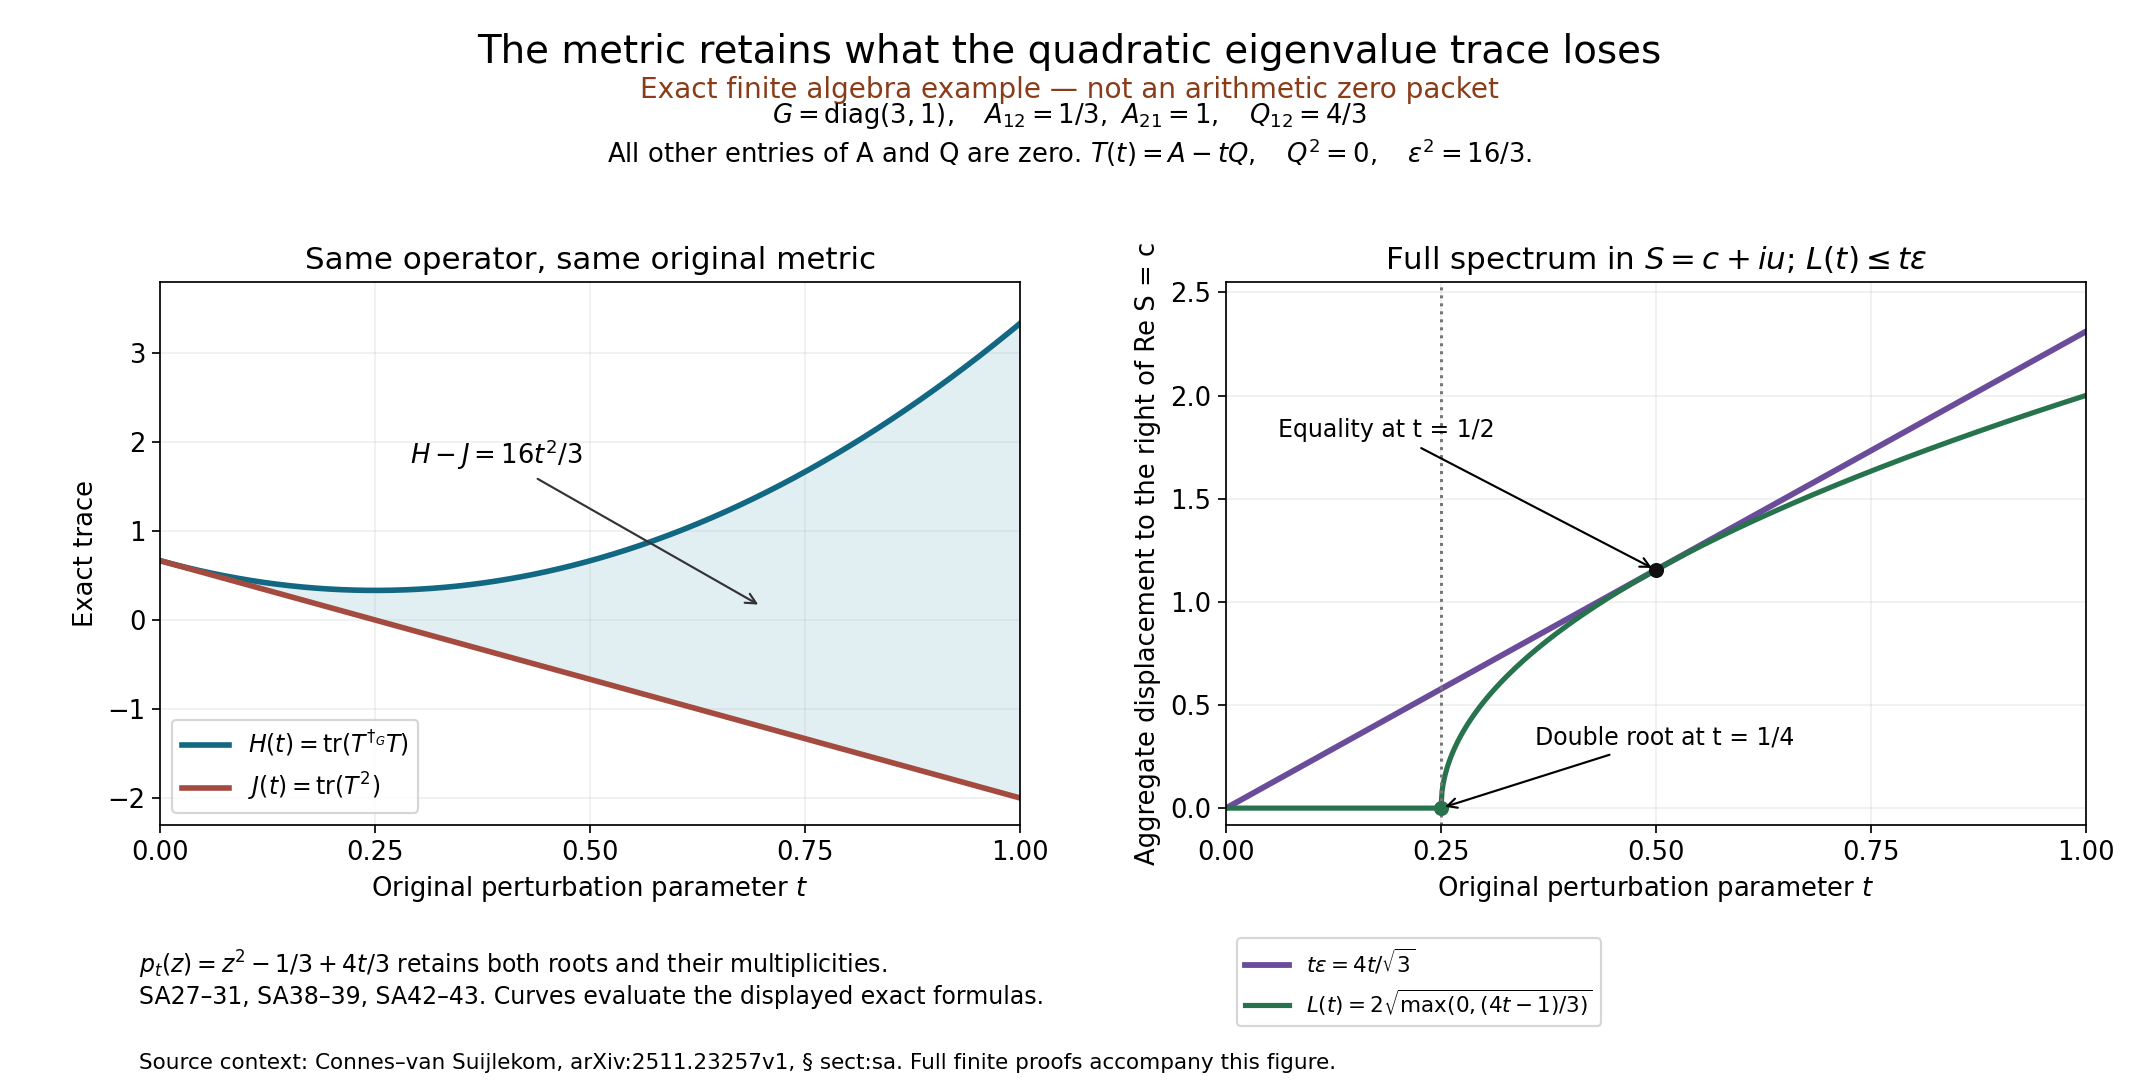
\includegraphics[width=\textwidth]{figures/metric_trace.png}
\end{center}
This is the mass-three uniform comparison measure on $[-1,1]$, not an
arithmetic zero packet. In its fixed metric $G=\operatorname{diag}(3,1)$,
$T(t)=A-tQ$ has $A_{12}=1/3$, $A_{21}=1$, $Q_{12}=4/3$ and all other
entries zero. The complete polynomial is $z^2-1/3+4t/3$.
The left panel retains the exact difference
$\operatorname{tr}(T^{\dagger_G}T)-\operatorname{tr}(T^2)=16t^2/3$.
The right panel uses the original coordinate $S=c+iu$ and counts both
roots with algebraic multiplicity. Its aggregate displacement is zero
up to $t=1/4$ and $2\sqrt{(4t-1)/3}$ thereafter, bounded by $4t/\sqrt3$,
with equality at $t=1/2$. These are the exact formulas proved in
SA27--31, SA38--39 and SA42--43, not sampled arithmetic zeros.
The human-source context is Connes and van Suijlekom,
\emph{Quadratic Forms, Real Zeros and Echoes of the Spectral Action},
\href{https://arxiv.org/abs/2511.23257v1}{arXiv:2511.23257v1},
Section \texttt{sect:sa}. All finite receiving formulas are proved above.
The figure generator and exact coordinates accompany this source.
\endgroup
% END COMPLETE NATIVE TRACE ACTION PROOFS
